\subsection{Prototype}

\textbf{Definición:} El patron prototype o prototipo tiene la finalidad de clonar nuevos objetos a partir de una instancia de objeto creada a priori. Para ello, el prototipo toma como base una estructura definida y realiza su clonación.

Un aspecto bastante importante que se debe tener en cuenta cuando se habla de clonación de objetos es que existen dos opciones al momento de clonar un objeto:

\begin{itemize}
	\item \textbf{Clonación superficial:} El proceso de instanciación se limita a crear una copia de los atributos de tipo primitivo (int, long, char, boolean, etc), por otro lado, los tipos de dato complejos son referenciados en la copia. Por lo tanto, si se realiza una modificación de un tipo de dato complejo en la copia, este afectará de manera directa al objeto original
	\item \textbf{Clonación profunda:} Se realiza una copia campo a campo del objeto original, resultando en que la copia es una instancia diferente miembro a miembro. Esto implica un costo de procesamiento mayor debido a que el sistema debe crear la estructura completa del objeto original. Sin embargo, modificar la copia no tendría ninguna consecuencia en el objeto original.
\end{itemize}


\textbf{Motivación:} En muchas ocasiones el costo de crear un nuevo objeto desde cero puede ser muy alto, en estas situaciones es adecuado clonar una estructura existente que actue como un prototipo y modifiar aquellos atributos que sean necesarios. Por otro lado, es posible que un usuario requiera crear una instancia identica de un objeto existente y no esté interesado en la manera en la cual se creó el objeto original. El patrón prototipo tiene la ventaja de ocultar la complejidad asociada a la creación de nuevas instancias.

\textbf{¿Como puedo implementar un prototype?:} El patrón prototipo delega la responsabilidad de clonar el objeto al objeto original a través de una interfaz común que se puede encargar de crear la copia del objeto. Generalmente, lenguajes orientados a objetos como JAVA permiten realizar la clonación mediante la implementación de la interfaz Cloneable que se encarga de realizar todo el proceso de copiar todos los atributos a una nueva instancia.

\textbf{Escenarios de aplicación:}

\begin{itemize}
	\item Es necesario crear nuevas instancias de una clase compleja que cumplen con la misma estructura de un modelo base.
	\item Se requiere instanciar objetos con una estructura común
	\item Se requiere crear objetos idénticos en tiempo de ejecución.
	\item La aplicación necesita crear multiples objetos con las mismas características evitando un consumo excesivo de recursos.
\end{itemize}

\textbf{Modelo UML:}

El corazón del patrón se centra en la definición de una interfáz encargada de permitir que la clonación del objeto sea transparente para el cliente, a partir de esto es posible crear las implementaciones necesarias de acuerdo a las necesidades del desarrollo.

\begin{figure}[H]
	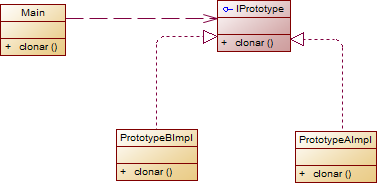
\includegraphics[width=0.9\textwidth]{images/creational/prototipe/prototype.png}
\end{figure}

\textbf{Ejemplo conceptual:} Científicos del instituto Roslin en Edimburgo lograron clonar el primer mamífero con éxito. Para ello se basaron en las células de una oveja finlandesa y tomaron su base genética como prototipo para obtener una oveja idéntica llamada Dolly. En este momento, se requiere realizar un programa computacional que emule este proceso a través de un proceso de clonación que permita al usuario clonar ovejas y conocer sus características individuales.

De acuerdo a las condiciones presentadas durante el experimento, existe una oveja que actua como prototipo a ser clonado, esto se puede lograr mediante la creación de una interfaz encargada de crear una copia exacta del objeto. Para ello, JAVA dispone de la interfaz Cloneable que permite realizar este proceso de manera transparente al usuario.

\begin{figure}[H]
	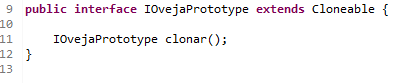
\includegraphics{images/creational/prototipe/prorotypeExample1.png}
\end{figure}

Tomando la interfaz como base, es posible crear nuevas ovejas mediante implementaciones específicas que ocupen el método clonar.

\begin{figure}[H]
	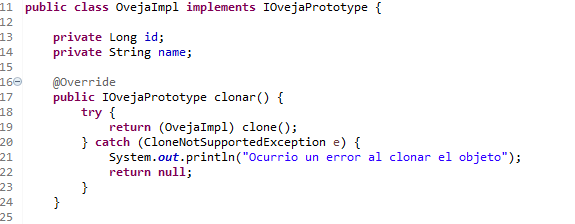
\includegraphics{images/creational/prototipe/prorotypeExample2.png}
\end{figure}

Adicionalmente, se sobreescribe el método toString() para presentar al usuario las propiedades básicas de la oveja.

\begin{figure}[H]
	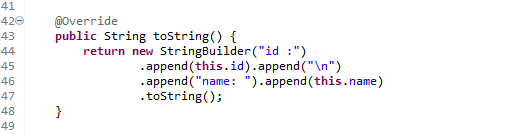
\includegraphics{images/creational/prototipe/prorotypeExample3.png}
\end{figure}

Finalmente, se implementa un cliente que permita a un usuario crear la oveja original y clonar las ovejas que desee. Para ello, el cliente crea una oveja original con sus características y posteriormente crea una copia exacta.

\begin{figure}[H]
	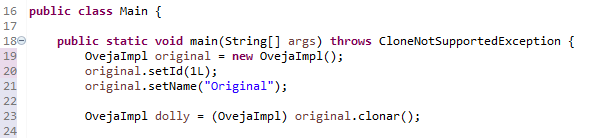
\includegraphics{images/creational/prototipe/prorotypeExample4.png}
\end{figure}

Como se puede observar, el patrón cumplió con su propósito creando una copia exacta de la oveja original

\begin{figure}[H]
	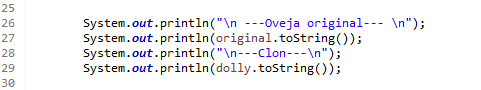
\includegraphics{images/creational/prototipe/prorotypeExample5.png}
\end{figure}

\begin{figure}[H]
	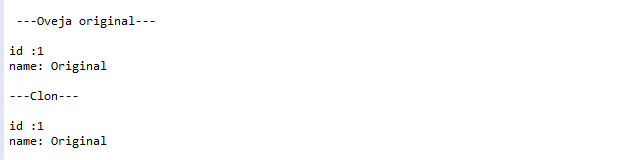
\includegraphics{images/creational/prototipe/prorotypeExample6.png}
\end{figure}

Sin embargo, a pesar que las ovejas tienen la misma información  no son el mismo objeto, por lo cual modificar la copia no afectará a la oveja original.

\begin{figure}[H]
	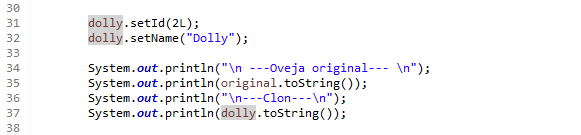
\includegraphics{images/creational/prototipe/prorotypeExample7.png}
\end{figure}

\begin{figure}[H]
	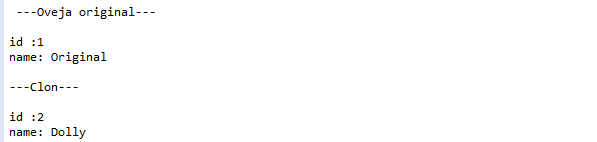
\includegraphics{images/creational/prototipe/prorotypeExample8.png}
\end{figure}

Debido a que las ovejas no son iguales, se puede concluir que hacen referencia a objetos diferentes en la aplicación.

\begin{figure}[H]
	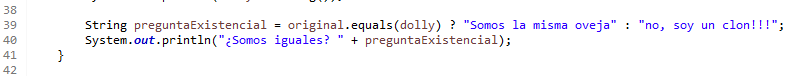
\includegraphics{images/creational/prototipe/prorotypeExample9.png}
\end{figure}

\begin{figure}[H]
	
\includegraphics{images/creational/prototipe/prorotypeExample10.png}
\end{figure}